% $Id$

\chapter{Building and Installing CUTS}
\label{chap:install}

CUTS has many small projects that comprise the entire system execution modeling
(SEM) tool. Its many projects, however, can be divided into three main categories, or
project groups:
\begin{itemize}
  \item Runtime architecture
  \item Modeling tools
  \item Analysis tools
\end{itemize}
This chapter discusses how to build and install each of the aforementioned
project groups for CUTS. Depending on your usage of CUTS, you may not need to build 
and install all projects in a category on the same machine. For example, you may install the 
runtime architecture of CUTS in your testing environment, and the modeling and analysis
tools outside of your testing environment to minimize interference with the testing 
process when viewing collected performance metrics in real-time. We are aware of 
these needs, and have setup the build process to decouple projects within a group from 
projects external to its corresponding category. You can, therefore, refer to each of the 
following sections on building and installation in isolation since project groups do 
not explicitly depend on each other.

\section{CUTS Runtime Architecture}
\label{sec:install-runtime}

The runtime architecture for CUTS allows developers and testers to emulate system 
experiments on their target architecture. CUTS also provides the mechanisms
to monitor and collect performance metrics for the executing system. In order to 
build the CUTS runtime architecture, you will need the following technologies 
installed on the target machine(s):
\begin{figure}[htbp]
  \centering
  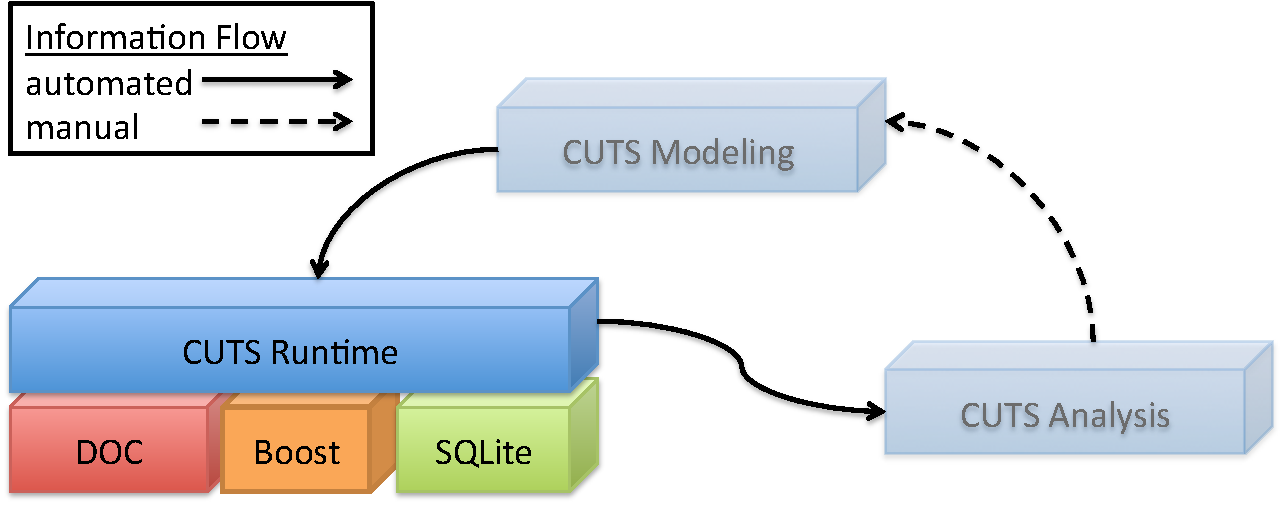
\includegraphics[scale=0.5]{cuts-runtime-blocks.pdf}
  \caption{Building blocks for the CUTS runtime architecture}
  \label{fig:cuts-runtime-blocks}
\end{figure}

\begin{itemize} 
  \item \textbf{ACE + TAO} - This set of middleware is used to abstract away the 
  complexities of implementing applications that operate on many different operating
  systems (ACE), and perform distributed communication (TAO). You can download ACE + TAO
  from the following location: \url{http://www.dre.vanderbilt.edu/TAO}.

  \item \textbf{Boost} - This set of libraries is used for implementing the parsers 
  (Boost Spirit) used within different artifacts of CUTS. You can download Boost from
  the following location: \url{http://www.boost.org}.

  \item \textbf{SQLite} - This set of libraries is used to support flat file archives
  for test results. You can download SQLite at the following location: 
  \url{http://www.sqlite.org}.

  \item \textbf{PCRE (not pictured)} - This set of libraries is used to enable PERL 
  regular expression support in CUTS. You can download PCRE at the following location:
  \url{http://www.pcre.org}.

  \item \textbf{XSC (not pictured)} - This set of libraries and applications is used to 
  convert XML documents to/from objects. You can download XSC from the following location: 
  \url{svn://svn.dre.vanderbilt.edu/XSC/trunk}.
\end{itemize}

\subsection{Obtaining Source Files}
\label{sec:install-download-runtime}

You can obtain the latest snapshot of the CUTS runtime architecture from the
DOC Group Subversion repository at the following location:
\begin{lstlisting}
(*@\url{svn://svn.dre.vanderbilt.edu/DOC/CUTS/trunk/CUTS}@*)
\end{lstlisting}
If you need to download a stable version of the source code, then you can 
access at one of the subdirectories in the repository at the following location:
\begin{lstlisting}
(*@\url{svn://svn.dre.vanderbilt.edu/DOC/CUTS/tags}@*)
\end{lstlisting}

\subsection{System Configuration}

Before you can build CUTS, you must for configure you environment. Please
set the following environment variables:
\begin{lstlisting}
(*@\texttt{\%> export CUTS\_ROOT=} location of CUTS@*)
(*@\texttt{\%> export LD\_LIBRARY\_PATH=\$LD\_LIBRARY\_PATH:\$CUTS\_ROOT/lib}@*)
(*@\texttt{\%> export PATH=\$PATH:\$CUTS\_ROOT/bin}@*)
\end{lstlisting}
Please see Appendix~\ref{chap:thirdparty} for instructions for configuring,
building, and installing third-party libraries needed by CUTS.

\subsection{Installation}

We use Makefile, Workspace, Project Creator (MPC)~\footnote{For more information
on MPC, please see the following location: \url{http://www.ociweb.com/products/mpc}}
to assist in building CUTS
on different operating systems, and with different compilers. Before you can
build the runtime architecture, you must first generate the target workspace.
Use the following command to generate the workspace:
\begin{lstlisting}
(*@\texttt{\%> \$(ACE\_ROOT)/bin/mwc.pl -type TYPE [-features FEATURES] CUTS.mwc}@*)
\end{lstlisting}
where TYPE is your compiler type, and FEATURES is a comma-separated list of 
enabled/disabled features
for your build of the CUTS runtime architecture.\footnote{You can type 
\texttt{\$ACE\_ROOT/bin/mwc.pl --help} to view the command-line options for 
MPC.} The complete set of features for CUTS is located in the following
file:
\begin{lstlisting}
(*@\texttt{\%> \$CUTS\_ROOT/default.features.tmpl}@*)
\end{lstlisting}
It is recommended that you copy the file above to the following location:
\begin{lstlisting}
(*@\texttt{\%> \$CUTS\_ROOT/default.features}@*)
\end{lstlisting}
and enable/disable the appropriate features for your workspace by 
modifying \texttt{default.features} accordingly. This way you do not
have to use the \texttt{-features} command-line option unless you want
to override your default feature selection. Once you have generated 
the workspace, you can build the solution using your specified compiler.

\section{CUTS Modeling Tools (Windows-only)}

CUTS modeling tools provide system developers and testers with an enviroment
for rapidly constructing experiments for distributed component-based systems,
and generating testing system for their target architecture. The modeling
tools are built on the following technologies:
\begin{figure}[htbp]
  \centering
  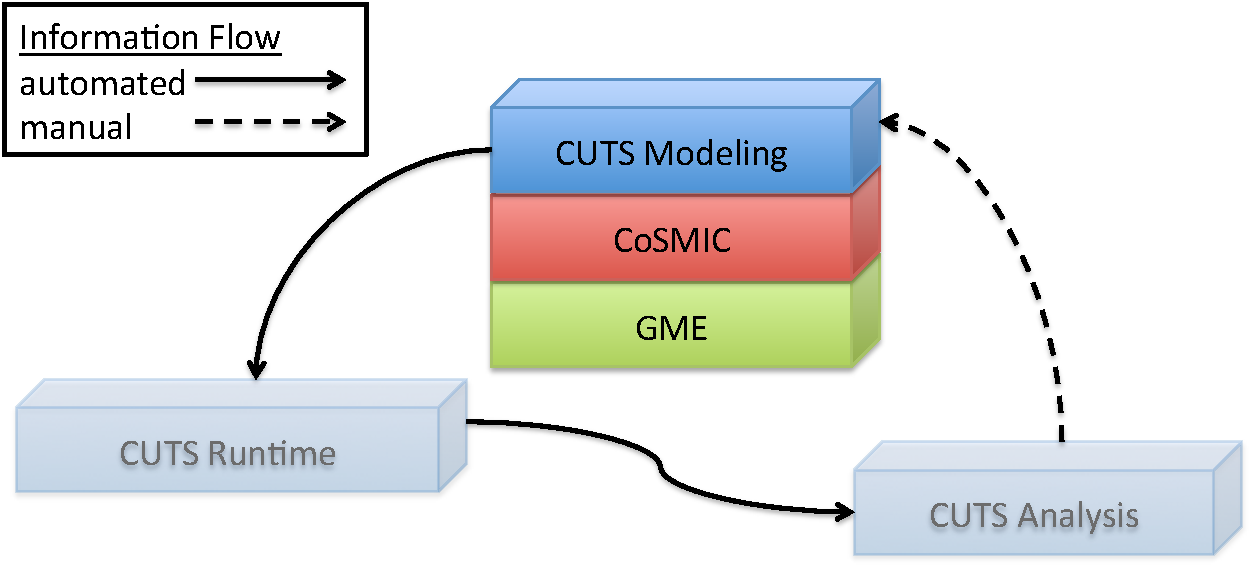
\includegraphics[scale=0.5]{cuts-modeling-blocks.pdf}
  \caption{Building blocks for the CUTS modeling tools}
  \label{fig:cuts-modeling-blocks}
\end{figure}

\begin{itemize}
  \item \textbf{GME} - The Generic Modeling Environment (GME) is a graphical
  modeling tool for creating domain-specific modeling languages (DSMLs). You
  can download GME from the following location: \url{http://www.isis.vanderbilt.edu/projects/GME}.

  \item \textbf{CoSMIC} - The Component Synthesis via Model Integrated 
  Computing (CoSMIC) is a tool suite designed to address the complexities of
  building large-scale component-based systesm, such as sytem assembly, 
  deployment, packaging, and planning. You can download CoSMIC from the following
  location: \url{http://www.dre.vanderbilt.edu/cosmic}.
\end{itemize}

\subsection{Installing Prebuilt Version}

The easiest and quickest way to install the CUTS modeling tools is to install
them using the .msi installer. You can download the latest version of the 
CUTS modeling tools from the following location:~\url{http://www.dre.vanderbilt.edu/CUTS/downloads}.
Before you can install the CUTS modeling tools, please make sure you have
installed GME and CoSMIC. Once both GME and CoSMIC are installed (in that
order), then you can install the CUTS modeling tools.

\subsection{Building from Sources (advanced)}

If you choose, you can build the modeling tools from source. This is given you
have downloaded all the source from the CUTS source code repository (see 
Section~\ref{sec:install-download-runtime}). To build the CUTS modeling tools,
first install the latest version of GME. Then, you \textbf{MUST} build CoSMIC
from source as well. This is required because the CUTS modeling tools are
built on top of CoSMIC, and its therefore dependent on CoSMIC. You can find
instructions for building CoSMIC from source at the following location:
\begin{lstlisting}
(*@\url{http://www.dre.vanderbilt.edu/cosmic/downloads}@*)
\end{lstlisting}
After you have built and installed CoSMIC from sources, you are ready to build
the CUTS modeling tools from source. Please use the following commands to 
build the modeling tools using your flavor of Visual C++:
\begin{lstlisting}
(*@\texttt{\%> cd \%CUTS\_ROOT\%}@*)
(*@\texttt{\%> mwc.pl -type [vc71 | vc8 | vc9] -features modeling=1,cosmic=1,boost=1,xsc=1,xscrt=1 CUTS\_CoSMIC.mwc}@*)
(*@\texttt{\%> open solution and build}@*)
\end{lstlisting}
The build process will ensure that all the interpreters are installed
and configured for your environment.

\section{CUTS Analysis Tools (Windows-only)}

The CUTS analysis tools allow developers to view and analyze performance metrics
of their system, and a CUTS test run. The analysis tools are built using the 
following key technologies:
\begin{figure}[htbp]
  \centering
  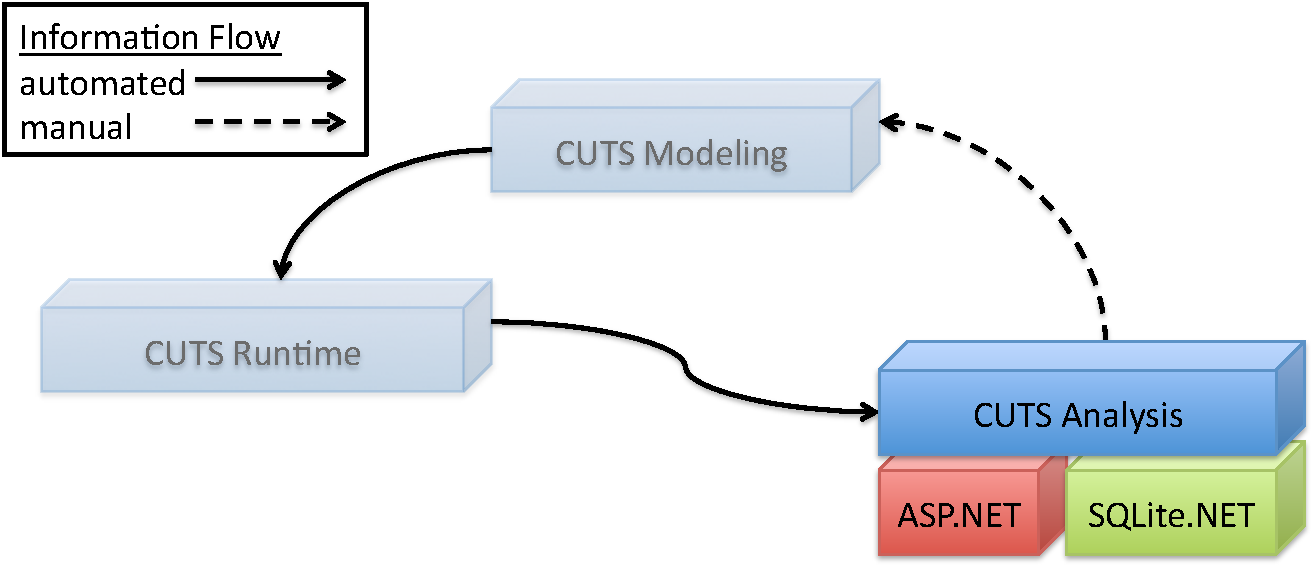
\includegraphics[scale=0.5]{cuts-analysis-blocks.pdf}
  \caption{Building blocks for the CUTS analysis tools}
  \label{fig:cuts-analysis-blocks}
\end{figure}
\begin{itemize}
  \item \textbf{ASP.NET} - ASP.NET is used to create the web application
  for the analysis tools, which is the main access portal for viewing 
  test results.

  \item \textbf{SQLite.NET} - SQLite.NET is the embedded database technology
  we use to manage the backend database(s). You can download SQLite.NET
  from the following location:~\url{http://sqlite.phxsoftware.com}
\end{itemize}

\subsection{Installing Prebuilt Version}

The easiest and quickest way to install the CUTS analysis tools is to install
them using the .msi installer. You can download the latest version of the
CUTS analysis tools from the following location:
\begin{lstlisting}
(*@~\url{http://www.dre.vanderbilt.edu/CUTS/downloads}@*)
\end{lstlisting}
Before you can install the CUTS modeling tools, please make sure you have
installed ASP.NET 2.0 and SQLite.NET. Once both ASP.NET 2.0 and SQLite.NET are 
installed, then you can install the CUTS modeling tools.~\footnote{We assume that 
Microsoft Internet Information Services (IIS) is already installed on the server
that you installing the CUTS analysis tools. Otherwise, please install Microsoft
IIS before installing the CUTS analysis tools, or any of its dependencies.}~\footnote{We
currently do not support Mono. Future versions of the CUTS analysis tools, however, will
support Mono.}

\subsection{Building from Sources (advanced)}

If you choose, you can build the CUTS analysis tools from source. This is given 
you have downloaded all the source from the CUTS source code repository (see
Section~\ref{sec:install-download-runtime}). To build the CUTS analysis tools,
first install Visual Studio.NET 2003 or better. Afterwards, please use the following 
commands to build the analysis tools:
\begin{lstlisting}
(*@\texttt{\%> cd \%CUTS\_ROOT\%$\backslash$utils$\backslash$BMW}@*)
(*@\texttt{\%> mwc.pl -type [vc8 | vc9] BMW.mwc}@*)
(*@\texttt{\%> open solution and build}@*)
\end{lstlisting}
The build process will ensure that all assemblies and the website build correctly. 
Once the build process is complete, you will to register the following location
with Microsoft IIS: \texttt{\%CUTS\_ROOT\%$\backslash$utils$\backslash$BMW$\backslash$website}.
This will allow you to view the website from your favorite web browser.
